\documentclass[pdflatex,compress]{beamer}

%\usetheme[dark,framenumber,totalframenumber]{ElektroITK}
\usetheme[darktitle,framenumber,totalframenumber]{ElektroITK}
\usepackage{graphicx}
\usepackage{multicol}

\title{Data Communications}
\subtitle{Chapter 3 - Data Transmission}

\author{Mifta Nur Farid, M.T.}

\begin{document}

\maketitle

\begin{frame}
	\frametitle{Transmission Terminology}
	\begin{itemize}
		\item Data transmission occurs between transmitter and receiver over some transmission medium
		\item Communication is in the form of electromagnetic waves
		\item Guided media: Twisted pair, coaxial cable, optical fiber
		\item Unguided media (wireless): Propagation through air, vacuum, and seawater
	\end{itemize}
\end{frame}

\begin{frame}{Transmission Terminology}
	\begin{itemize}
		\item Direct link:
		\begin{itemize}
			\item No intermediate devices other than amplifiers or repeater used to increase signal strength.
		\end{itemize}
		\item Point-to-point: 
		\begin{itemize}
			\item Direct link between two devices
			\item Only 2 devices sharing medium
		\end{itemize}
		\item Multi-point
		\begin{itemize}
			\item More than two devices share the same medium
		\end{itemize}
	\end{itemize}
\end{frame}

\begin{frame}{Transmission Terminology}
	\begin{itemize}
		\item Simplex
		\begin{itemize}
			\item Signals are transmitted in only one direction
			\item One station is transmitter and the other is
			receiver
		\end{itemize}
		\item Half duplex 
		\begin{itemize}
			\item Both stations transmit, but only one at a time
		\end{itemize}
		\item Full duplex
		\begin{itemize}
			\item Both stations may transmit simultaneously
			\item The medium is carrying signals in both directions at the same time
		\end{itemize}
	\end{itemize}
\end{frame}

\begin{frame}
	\begin{center}
		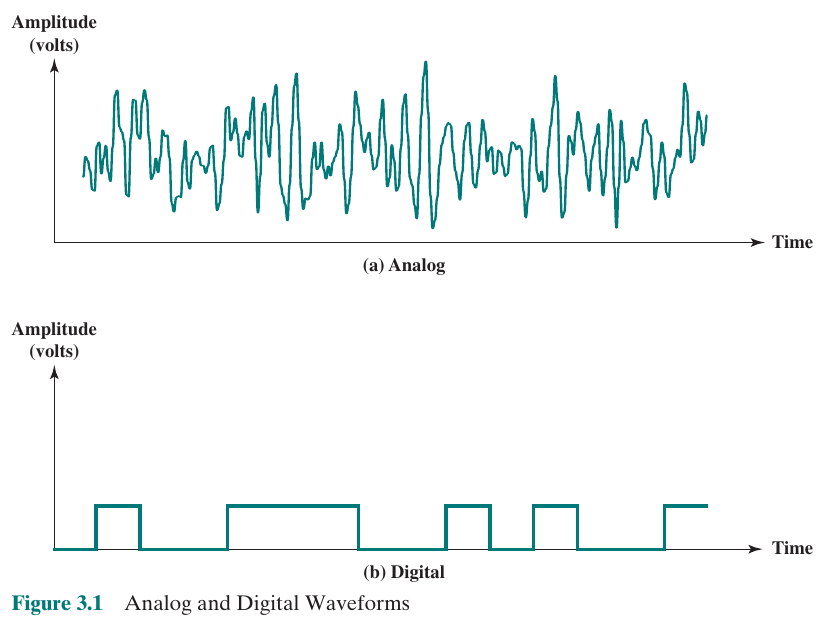
\includegraphics[width=0.9\linewidth]{img/img01}
	\end{center}
\end{frame}

\begin{frame}
	\begin{center}
		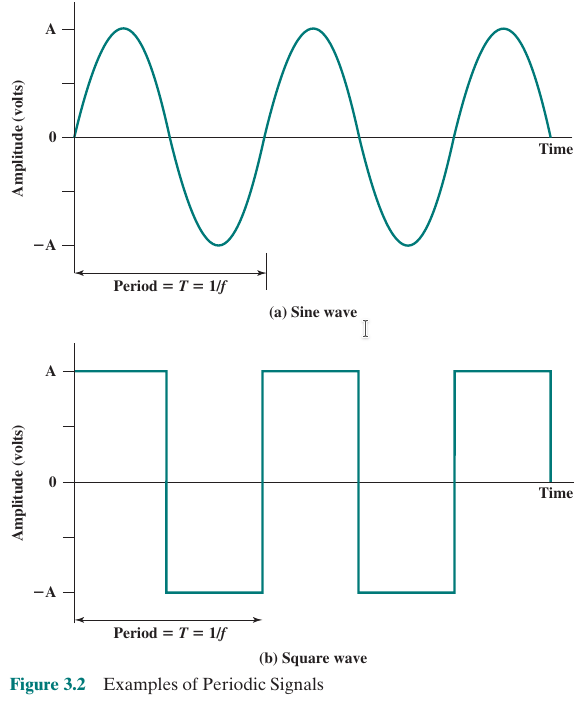
\includegraphics[height=0.9\textheight]{img/img02}
	\end{center}
\end{frame}

\begin{frame}
	\frametitle{Sine Wave}
	\begin{itemize}
		\item The fundamental periodic signal
		\item Can be represented by three parameters
		\begin{itemize}
			\item Peak amplitude (A)
			\begin{itemize}
				\item Maximum value or strength of the signal over time
				\item Typically measured in volts
			\end{itemize}
			\item Frequency (f)
			\begin{itemize}
				\item Rate at which the signal repeats
				\item Hertz (Hz) or cycles per second
				\item Period (T) is the amount of time for one repetition
				\item T = 1/f
			\end{itemize}
			\item Phase ($ \phi $)
			\begin{itemize}
				\item Relative position in time within a single period of signal
			\end{itemize}
		\end{itemize}
	\end{itemize}
\end{frame}

\begin{frame}
	\begin{center}
		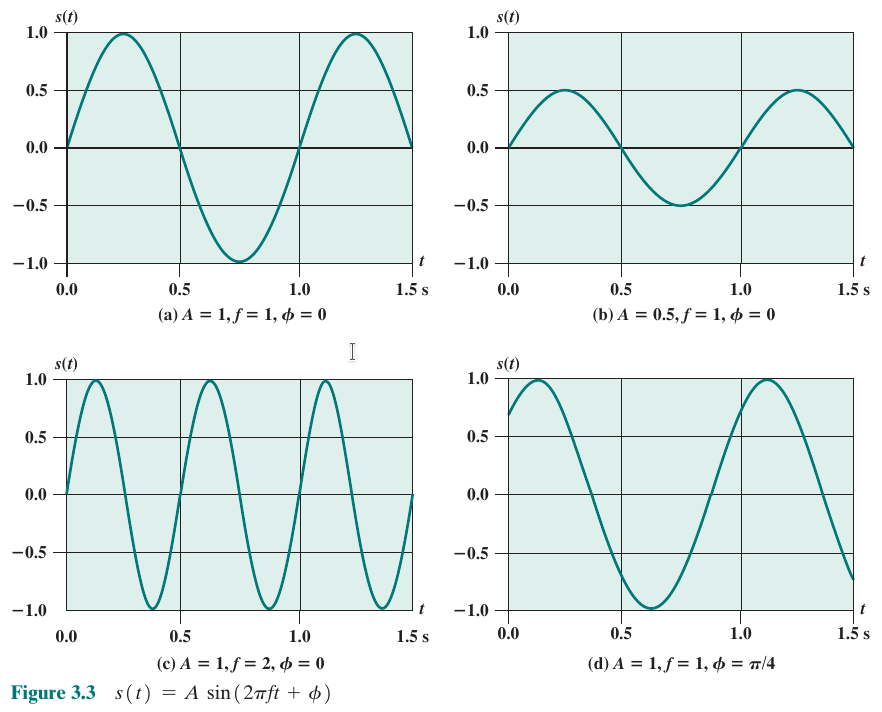
\includegraphics[height=0.9\textheight]{img/img03}
	\end{center}
\end{frame}

\begin{frame}
	\frametitle{Wavelength ($ \lambda $)}
	\begin{itemize}
		\item The wavelength of a signal is the distance occupied by a single cycle
		\item Can also be stated as the distance between two points of corresponding phase of two consecutive cycles
		\item Assuming signal velocity $ v $, then the wavelength is related to the period as $ \lambda = vT $
		\item Especially when $ v=c $\\
		$ c = 3\times10^8 $ m/s (speed of light in free space)
		\item Or equivalently $ \lambda f = v $
	\end{itemize}
\end{frame}

\begin{frame}
	\frametitle{Frequency Domain Concepts}
	\begin{itemize}
		\item Signals are made up of many frequencies
		\item Components are sine waves
		\item Fourier analysis can show that any signal is made up of components at various frequencies, in which each component is a sinusoid
		\item Can plot frequency domain functions
	\end{itemize}
\end{frame}

\begin{frame}
	\begin{center}
		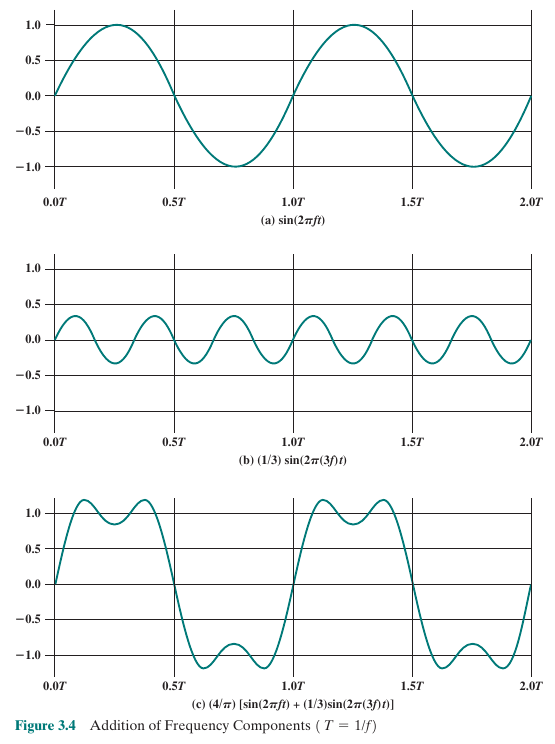
\includegraphics[height=0.9\textheight]{img/img04}
	\end{center}
\end{frame}

\begin{frame}
	\begin{center}
		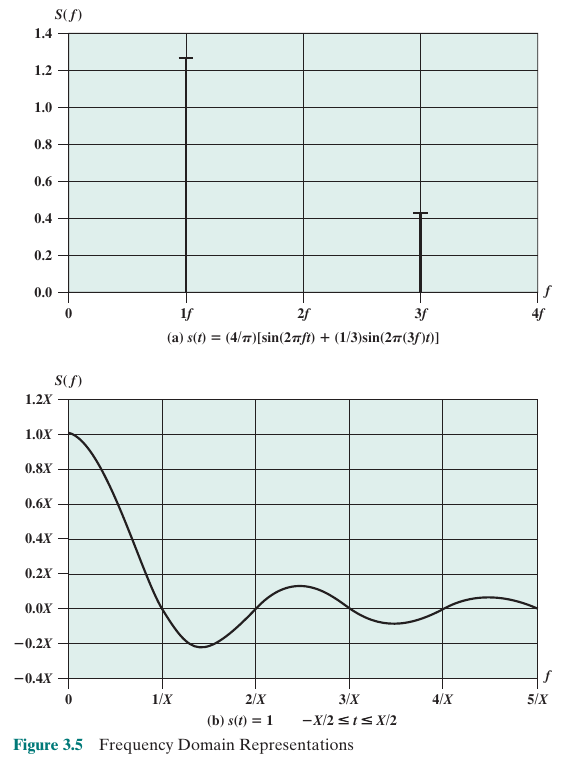
\includegraphics[height=0.9\textheight]{img/img05}
	\end{center}
\end{frame}

\begin{frame}
	\frametitle{Spectrum and Bandwidth}
	\begin{itemize}
		\item Spectrum: Range of frequencies contained in signal
		\item Absolute bandwidth: Width of spectrum
		\item Effective bandwidth (or just bandwidth): Narrow band of frequencies containing most energy
		\item DC Component: Component of zero frequency
	\end{itemize}
\end{frame}



\end{document}
